%% Figura standalone per la submission IEEE JBHI.
%% Compilare con: pdflatex fig3_scaling_sweep.tex -> PDF vettoriale, font incorporati.
%% Font Times (ptm) per corrispondere a ieeecolor.cls.
%% Larghezza di destinazione: colonna singola (figure, ~8.8 cm):
%% small multiples 2x2 anziche' quattro pannelli affiancati a piena pagina.
\documentclass[tikz,border=1pt]{standalone}
\renewcommand{\rmdefault}{ptm}
\usepackage{amsmath,amssymb}
\usetikzlibrary{positioning, arrows.meta, shapes.geometric}

%% Palette categoriale validata (slot 1 blu, slot 2 arancio).
\definecolor{serQwen}{HTML}{2A78D6}
\definecolor{serGemma}{HTML}{EB6834}
\definecolor{inkMuted}{HTML}{52514E}

\begin{document}
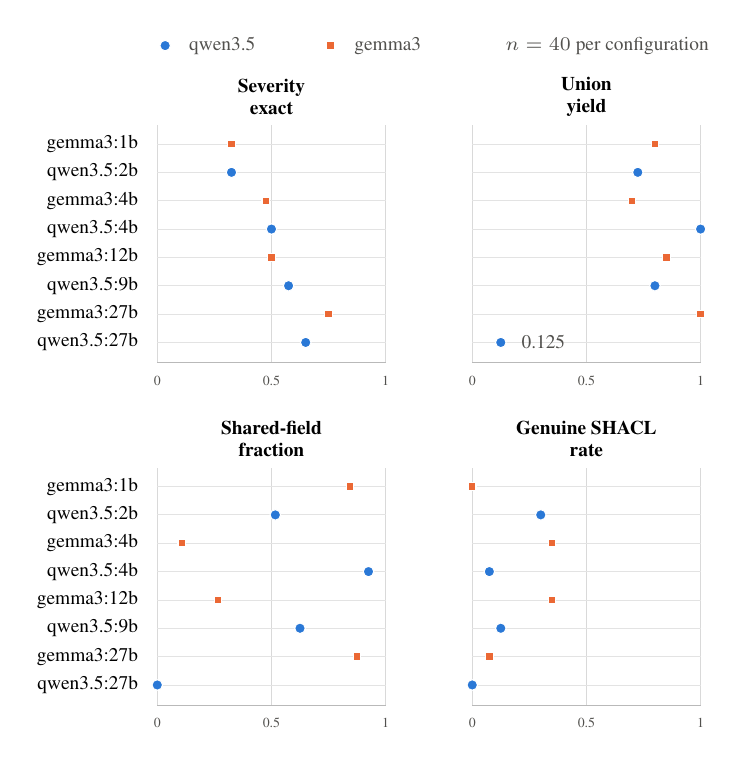
\begin{tikzpicture}[
  qwenmark/.style={circle, fill=serQwen, draw=white, line width=0.4pt, inner sep=1.35pt},
  gemmamark/.style={rectangle, fill=serGemma, draw=white, line width=0.4pt, inner sep=1.35pt},
  scaletick/.style={font=\scriptsize, text=inkMuted},
  scalemodel/.style={font=\scriptsize, anchor=east},
  scalepanel/.style={font=\scriptsize\bfseries, align=center},
  callout/.style={font=\scriptsize, text=inkMuted, anchor=west}
]
  %% --- geometria (unita': cm) ---
  \def\pw{2.90}              % larghezza pannello (0--1)
  \def\colb{4.00}            % origine x della seconda colonna di pannelli
  \def\rowsep{0.36}          % passo verticale fra modelli
  \def\blockb{-4.35}         % scostamento y del blocco inferiore
  \pgfmathsetmacro{\ytop}{7*\rowsep}

  %% --- griglia, assi e intestazione di un pannello ---
  %% Macro anziche' \foreach: il titolo contiene \\ per l'andata a capo,
  %% che \foreach non gestisce all'interno degli elementi della lista.
  \newcommand{\drawpanel}[3]{%
    \foreach \tv/\lab in {0/0, 0.5/0.5, 1/1} {
      \pgfmathsetmacro{\xx}{#1+\tv*\pw}
      \draw[gray!30, line width=0.25pt]
        (\xx,{#2-0.26}) -- (\xx,{#2+\ytop+0.24});
      \node[scaletick, below, font=\tiny] at (\xx,{#2-0.30}) {\lab};
    }
    \draw[gray!55, line width=0.4pt] (#1,{#2-0.26}) -- ({#1+\pw},{#2-0.26});
    \node[scalepanel] at ({#1+\pw/2},{#2+\ytop+0.60}) {#3};
  }
  \drawpanel{0}{0}{Severity\\exact}
  \drawpanel{\colb}{0}{Union\\yield}
  \drawpanel{0}{\blockb}{Shared-field\\fraction}
  \drawpanel{\colb}{\blockb}{Genuine SHACL\\rate}

  %% --- righe: un marker per modello in ciascun pannello ---
  %% Modelli ordinati per numero di parametri crescente, famiglie alternate:
  %% cosi' la non monotonicita' dell'union yield si legge scorrendo dall'alto.
  \foreach \name/\marker/\severity/\union/\shared/\genuine [count=\i from 0] in {
    gemma3:1b/gemmamark/0.325/0.800/0.844/0.000,
    qwen3.5:2b/qwenmark/0.325/0.725/0.517/0.300,
    gemma3:4b/gemmamark/0.475/0.700/0.107/0.350,
    qwen3.5:4b/qwenmark/0.500/1.000/0.925/0.075,
    gemma3:12b/gemmamark/0.500/0.850/0.265/0.350,
    qwen3.5:9b/qwenmark/0.575/0.800/0.625/0.125,
    gemma3:27b/gemmamark/0.750/1.000/0.875/0.075,
    qwen3.5:27b/qwenmark/0.650/0.125/0.000/0.000
  } {
    \pgfmathsetmacro{\yy}{7*\rowsep-\i*\rowsep}
    %% etichette del modello: una volta per blocco (asse y condiviso in riga)
    \node[scalemodel] at (-0.12,\yy) {\name};
    \node[scalemodel] at (-0.12,{\blockb+\yy}) {\name};

    \foreach \ox/\oy in {0/0, \colb/0, 0/\blockb, \colb/\blockb} {
      \draw[gray!22, line width=0.3pt] (\ox,{\oy+\yy}) -- ({\ox+\pw},{\oy+\yy});
    }

    \node[\marker] at ({\severity*\pw},\yy) {};
    \node[\marker] at ({\colb+\union*\pw},\yy) {};
    \node[\marker] at ({\shared*\pw},{\blockb+\yy}) {};
    \node[\marker] at ({\colb+\genuine*\pw},{\blockb+\yy}) {};
  }

  %% --- etichetta diretta selettiva: l'outlier discusso nel testo ---
  \pgfmathsetmacro{\yout}{7*\rowsep-7*\rowsep}
  \node[callout] at ({\colb+0.125*\pw+0.14},\yout) {0.125};

  %% --- legenda ---
  \pgfmathsetmacro{\ylg}{\ytop+1.25}
  \node[qwenmark] at (0.10,\ylg) {};
  \node[scaletick, anchor=west] at (0.28,\ylg) {qwen3.5};
  \node[gemmamark] at (2.20,\ylg) {};
  \node[scaletick, anchor=west] at (2.38,\ylg) {gemma3};
  \node[scaletick, anchor=west] at (4.30,\ylg) {$n=40$ per configuration};
\end{tikzpicture}
\end{document}
